% One-page A4 CV. Build: pdflatex CV_A4.tex (cvmfs TeX Live 2025)
\documentclass[10pt]{article}
\usepackage[a4paper,left=1.45cm,right=1.45cm,top=1.1cm,bottom=0.9cm]{geometry}
\usepackage[T1]{fontenc}
\usepackage[utf8]{inputenc}
\usepackage[default,semibold]{sourcesanspro}
\usepackage{sourceserifpro}
\usepackage{xcolor,graphicx,tikz,enumitem,tabularx}
\usepackage[expansion=false]{microtype}
\usepackage[hidelinks]{hyperref}

\definecolor{navy}{HTML}{194E89}
\definecolor{accent}{HTML}{C05719}
\definecolor{muted}{HTML}{5F6B7A}
\definecolor{rulegray}{HTML}{D9DEE6}
\definecolor{ink}{HTML}{1F2933}

\pagestyle{empty}
\setlength{\parindent}{0pt}
\linespread{1.05}
\hyphenpenalty=10000 \exhyphenpenalty=10000 \tolerance=2000 \emergencystretch=2em
\color{ink}

\newcommand{\org}[1]{\textcolor{navy}{#1}}
\newcommand{\sep}{\,\textcolor{muted}{·}\,}
\newcommand{\dates}[1]{\hfill\textcolor{muted}{#1}}

% section heading: orange square, spaced navy capitals, grey rule
\newcommand{\cvsection}[1]{%
  \par\vspace{6pt}%
  {\color{accent}\rule{5pt}{5pt}}\hspace{6pt}%
  {\color{navy}\bfseries\small\textls[180]{\MakeUppercase{#1}}}\hspace{6pt}%
  {\color{rulegray}\leaders\hrule height 0.6pt depth 0pt\hfill}\par\vspace{4pt}}

% entry: bold role · navy organisation · extra, dates right
\newcommand{\entry}[4]{\par\vspace{3pt}\textbf{#1}\sep\org{#2}#3\dates{#4}\par}
\setlist[itemize]{leftmargin=13pt,itemsep=0pt,topsep=1pt,parsep=0pt,label=\textbullet}
\setlist[enumerate]{leftmargin=18pt,itemsep=0pt,topsep=1pt,parsep=1pt}

\begin{document}
\raggedright

% ---------------- header ----------------
\begin{minipage}[c]{2.45cm}
  \begin{tikzpicture}
    \clip[rounded corners=4pt] (0,0) rectangle (2.4cm,3.19cm);
    \node[anchor=south west,inner sep=0] at (0,0) {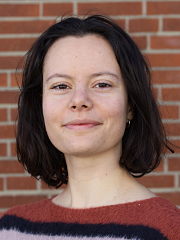
\includegraphics[width=2.4cm,height=3.19cm]{photo_color.jpg}};
  \end{tikzpicture}
\end{minipage}\hspace{0.45cm}%
\begin{minipage}[c]{\dimexpr\linewidth-2.9cm}
  {\fontsize{25}{28}\selectfont\fontfamily{SourceSerifPro-TLF}\selectfont\bfseries\color{navy}Martina Mozzanica}\par\vspace{5pt}
  {\bfseries PhD Candidate · Machine Learning for High Energy Physics}\par\vspace{5pt}
  {\small\textcolor{muted}{Hamburg, Germany}\hspace{1.2em}%
  \href{mailto:martina.mozzanica@gmail.com}{\org{martina.mozzanica@gmail.com}}\hspace{1.2em}%
  \href{https://www.linkedin.com/in/martina-mozzanica-20017b202}{\org{linkedin.com/in/martina-mozzanica}}}
\end{minipage}
\par\vspace{8pt}

\begin{tikzpicture}
  \fill[accent] (0,0) rectangle (0.1\linewidth,1.6pt);
  \fill[navy] (0.1\linewidth,0) rectangle (\linewidth,1.6pt);
\end{tikzpicture}

% ---------------- profile ----------------
\cvsection{Profile}
PhD candidate in generative machine learning at the University of Hamburg, building fast, geometry-independent calorimeter simulations with point-cloud generative models. Earlier work at CERN and Milano-Bicocca developed graph neural networks for the LHCb trigger. Experienced across the HEP software chain, from Geant4 and Key4hep to PyTorch training on GPU clusters.

% ---------------- research experience ----------------
\cvsection{Research Experience}
\entry{Research Stay}{CERN, Geneva}{}{May 2026 -- Jul 2026}
\begin{itemize}
  \item Built an end-to-end pipeline (Geant4 $\to$ Key4hep $\to$ step2point $\to$ CaloClouds3) to study how the choice of point-cloud representation affects a generative shower model for the ILD calorimeter.
\end{itemize}
\entry{PhD Candidate}{University of Hamburg}{}{Sep 2023 -- present}
\begin{itemize}
  \item Generative machine learning for high energy physics in the group of Prof.\ Gregor Kasieczka.
  \item Developed CaloHadronic, a diffusion model for hadronic showers across the electromagnetic and hadronic calorimeters, and CaloCHILL, which generates showers with hit times in a learned latent space, 600 times faster than its predecessor.
\end{itemize}
\entry{Research Fellow}{Università degli Studi di Milano-Bicocca}{}{Apr 2023 -- Jul 2023}
\begin{itemize}
  \item Continued master's thesis work: graph neural networks for the DFEI project at LHCb.
\end{itemize}
\entry{Research Stay}{CERN, Geneva}{\sep Deep Full Event Interpretation (DFEI) project, LHCb}{Jun 2023 -- Jul 2023}
\entry{Research Stay}{CERN, Geneva}{\sep Master's thesis with the DFEI group}{Oct 2022 -- Nov 2022}

% ---------------- education ----------------
\cvsection{Education}
\entry{PhD in Physics (ongoing)}{University of Hamburg}{}{Sep 2023 -- present}
\entry{M.Sc.\ in Physics, High Energy Physics}{Università degli Studi di Milano-Bicocca}{}{Oct 2020 -- Mar 2023}
Thesis: graph neural networks for the LHCb trigger, with the DFEI group at CERN.\par
\entry{Erasmus+ Exchange, Engineering Physics}{Technical University of Munich}{}{Oct 2021 -- Mar 2022}
\entry{B.Sc.\ in Physics, Applied Physics}{Università degli Studi dell'Insubria}{}{2017 -- 2020}

% ---------------- publications ----------------
\cvsection{Publications}
\begin{enumerate}
  \item \href{https://arxiv.org/abs/2304.08610}{GNN for Deep Full Event Interpretation and Hierarchical Reconstruction of Heavy-Hadron Decays in Proton--Proton Collisions} \href{https://arxiv.org/abs/2304.08610}{\textcolor{muted}{[2304.08610]}}
  \item \href{https://arxiv.org/abs/2501.05534}{OmniJet-$\alpha_{\textup{C}}$: Learning Point Cloud Calorimeter Simulations Using Generative Transformers} \href{https://arxiv.org/abs/2501.05534}{\textcolor{muted}{[2501.05534]}}
  \item \href{https://arxiv.org/abs/2506.21720}{CaloHadronic: A Diffusion Model for the Generation of Hadronic Showers} (lead author) \href{https://arxiv.org/abs/2506.21720}{\textcolor{muted}{[2506.21720]}}
  \item \href{https://arxiv.org/abs/2511.01460}{CaloClouds3: Ultra-Fast Geometry-Independent Highly-Granular Calorimeter Simulation} \href{https://arxiv.org/abs/2511.01460}{\textcolor{muted}{[2511.01460]}}
  \item \href{https://arxiv.org/abs/2606.11304}{SPADE: Split-and-Delay Embeddings for Autoregressive High-Granularity Calorimeter Simulation} \href{https://arxiv.org/abs/2606.11304}{\textcolor{muted}{[2606.11304]}}
  \item \href{https://arxiv.org/abs/2609.24306}{Jevons' Paradox and Fast Generative Simulation for HEP: Why Realistic Benchmarking Is Essential} \href{https://arxiv.org/abs/2609.24306}{\textcolor{muted}{[2609.24306]}}
  \item \href{https://arxiv.org/abs/2609.30403}{Point-Cloud Generative Models for Fast Calorimeter Simulation Across Particles and Geometries} \href{https://arxiv.org/abs/2609.30403}{\textcolor{muted}{[2609.30403]}}
  \item \href{https://arxiv.org/abs/2611.08606}{Just CaloCHILL: Fast Hadronic Shower Generation in a Learned Latent Space} (lead author) \href{https://arxiv.org/abs/2611.08606}{\textcolor{muted}{[2611.08606]}}
\end{enumerate}

% ---------------- skills ----------------
\cvsection{Skills}
\begin{tabularx}{\linewidth}{@{}p{3.2cm}>{\raggedright\arraybackslash}X@{}}
  \textbf{Machine learning} & Generative models, diffusion models, normalizing flows, VAEs, model distillation, transformers, graph neural networks, point-cloud models, HDBSCAN\\[1pt]
  \textbf{Programming} & Python, C++, PyTorch, TensorFlow\\[1pt]
  \textbf{HEP software} & Geant4, Key4hep, ROOT
\end{tabularx}

% ---------------- other experience ----------------
\cvsection{Other Experience}
\begin{itemize}
  \item \textbf{Substitute Teacher}, ISIS Valceresio\sep May 2021
  \item \textbf{Referee}, Centro Sportivo Italiano\sep 2016 -- 2017
  \item \textbf{Certified Artistic Gymnastics Judge}
\end{itemize}

\end{document}
